usepackage{graphicx}
\section{Evaluation}
\label{sec:eval}

The evaluation aims to answer the following questions:

\begin{itemize}
\item Does multi-dispatch linearizability offer applications significantly lower end-to-end latency for realistic workloads compared to baselines?

\item What are the limitations and main overheads of multi-dispatch linearizability?

\item Which programming styles benefit from interacting with an md-linearizable service and what applications could use multi-dispatch linearizability?
\end{itemize}

\subsection{Experimental Set-up}
We implement a MDL key-value store that uses MDL-Paxos per shard, and the multi-dispatch protocol for cross-shard coordination.
\begin{itemize}
    \item Using 5(3) replicas per shard
    \item Using 5(2) shards
    \item Cloudlab, replicas and shards within single data center, 10Gbs local network
    \item Each server is 10 cores, Intel Xeon Silver 4114, 2.2GHz
\end{itemize}
\subsection{End-to-end Application Latency}
\begin{figure}[!htb]
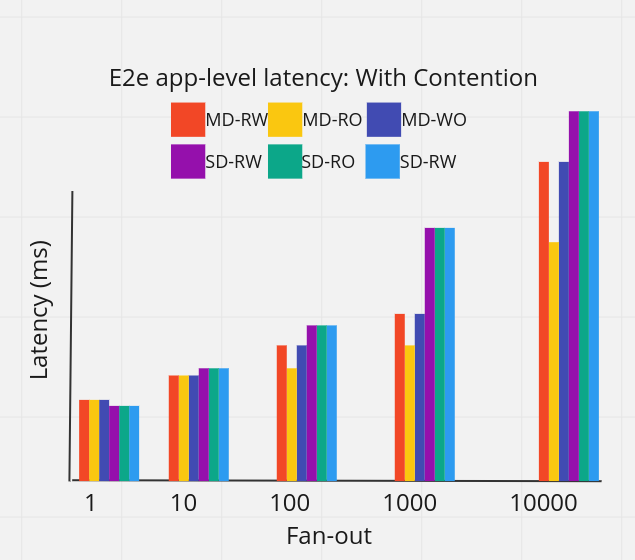
\includegraphics[scale=.32]{e2e-with-contention.png}
\caption{Multi-sharded MDL with high contention.}
\label{fig:e2e-contention}
\end{figure}
In this section, we show how the end-to-end application latency of mdl compares to sdl.
The variables we vary:
\begin{itemize}
    \item Skew (uniform vs. zipfian)
    \item Number of clients
    \item Types of requests - RW, WO, RO
    \item Fan-out
    \item Request arrival-time
    \item Inter-shard distance
    \item Network lossiness?
        \subitem This would highlight the overhead of buffering that happens with out of order packets for MD-lin, but it might not be interesting if the metric is e2e app-req latency
    \item Failure rate
\end{itemize}
To keep the load on the system the same between sdl and mdl, we increase the number of concurrent clients for sdl but keep it constant for mdl as the number of requests per client increases, keeping the overall number of requests sent to the system the same for both.

We also compare against different request types: read-only, write-only, and read-write. We expect to see a difference in performance for these since multiple read-only requests issued will never have conflicts, whereas the other two types can induce conflicts that lead to reissuing.

We look at two cases of interest, when there is high contention across the concurrent requests from different clients, and when there isn't. 

Figure \ref{fig:e2e-contention} shows that in the former case, we expect significant slow downs of multi-dispatch due to the reissuing of requests, which degrades very fast when there is high load on the system.

Figure \ref{fig:e2e-nocontention}, produced by distributing requests uniformly and keeping cross batch overlap minimal, shows that without contention, the system reorders requests much less frequently.
\begin{figure}[!htb]
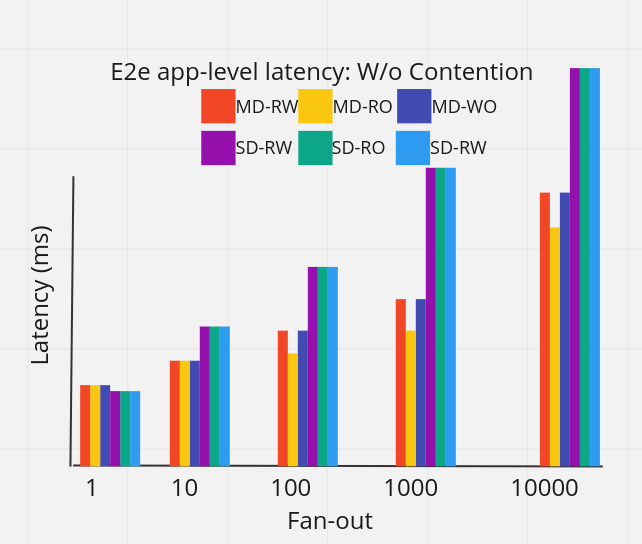
\includegraphics[scale=.32]{e2e-wo-contention.png}
\caption{Multi-sharded MDL with low contention.}
\label{fig:e2e-nocontention}
\end{figure}

\subsection{Protocol Performance Overheads}
In this section we measure the overhead of the multi-dispatch protocol.
\begin{figure}[!htb]
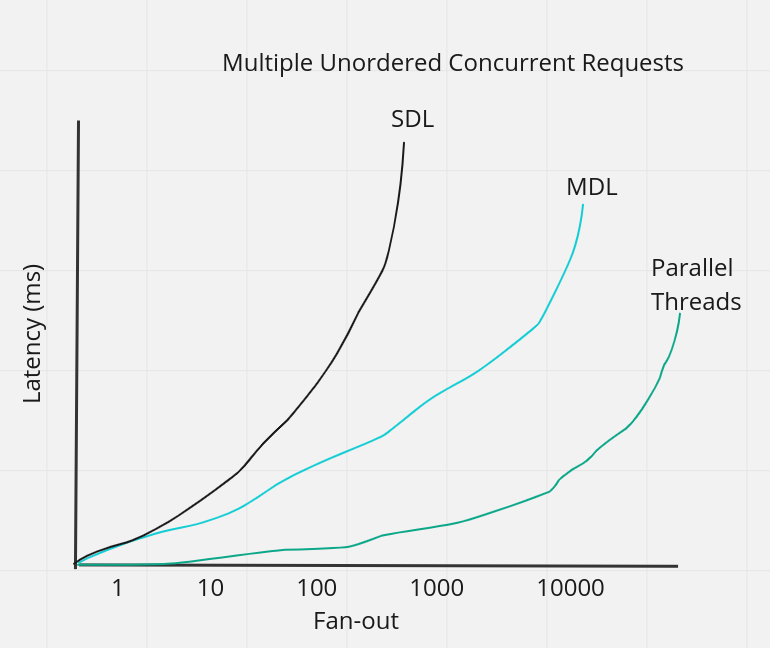
\includegraphics[scale=.27]{unordered_multithreaded.png}
\caption{Multi-threaded client without linearizability compared to multi-dispatch client with linearizability compared to single-dispatch client with linearizability.}
\label{fig:unordered-mt}
\end{figure}
\subsubsection{Correctness Overheads}
In figure \ref{fig:unordered-mt} we show the overhead induced for ensuring a linearizable ordering among requests issued by an application. We compare SDL and MDL as in the previous section, but we also add a third baseline that demonstrates the behavior of issuing all system-level requests for a single application level requests in parallel to a SDL backend. This method does not provide a consistent linearizable ordering, but can be faster than using MDL which pays an overhead to ensure issue-order.

Next, in figure \ref{fig:sequential-md} we show the slowdown incurred from conflict detection. A single-dispatch usage pattern of a MDL system is slower than the same usage on a SDL system, and this is due to the overhead of intershard coordination and conflict detection.

To run this experiment, we vary the number of clients, and measure the end-to-end latency of singly-issuing 10 requests to the backend.
\begin{figure}[!htb]
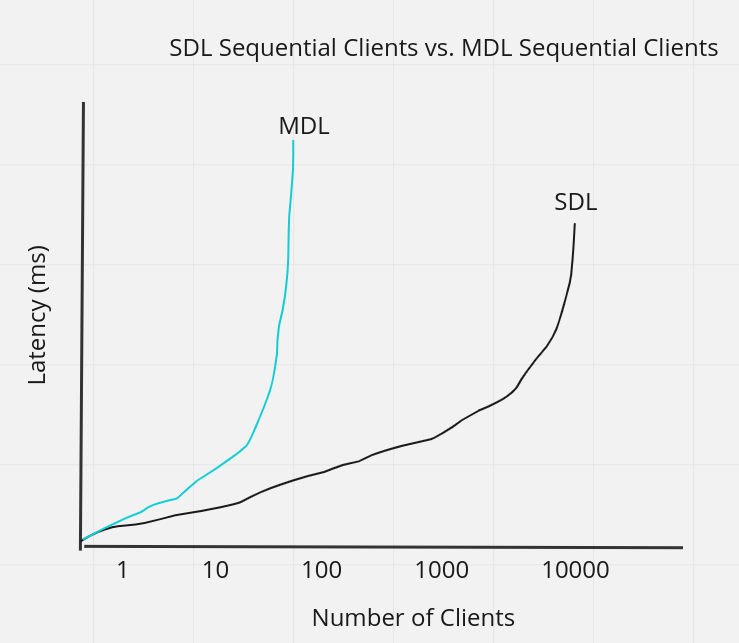
\includegraphics[scale=.27]{sequential_MDL.png}
\caption{We show the performance of issuing requests sequentially to a SDL system compared to a MDL system.}
\label{fig:sequential-md}
\end{figure}
\subsubsection{Single-shard vs. Multi-shard}
Run experiments with a single client on single shard and compare to multi-shard. In figure \ref{fig:ss-vs-ms}, we show that the performance improvement of single-sharded multi-dispatch over single-dispatch is much greater than the counterpart for multiple shards. This is because SDL is local, while MDL is not, so we must pay the price for inter-shard communication.
\begin{figure}[!htb]
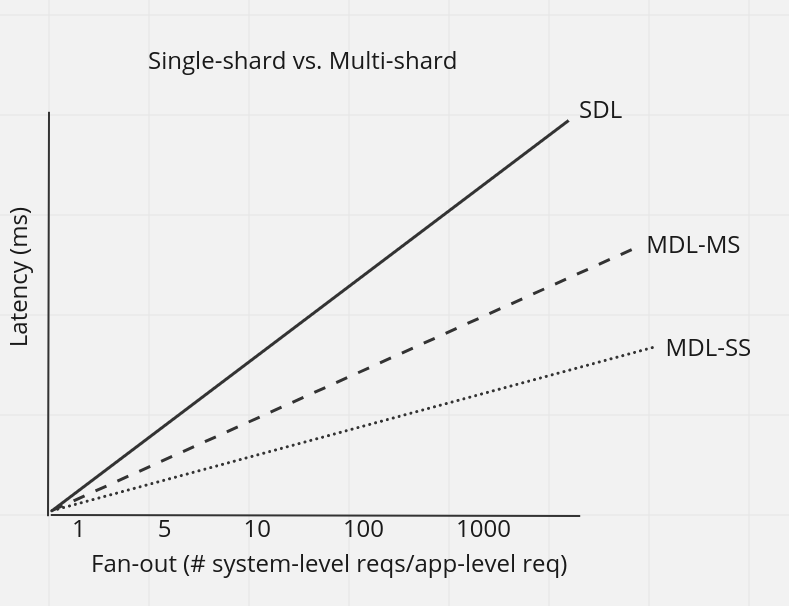
\includegraphics[scale=.27]{single-shard-multi-shard.png}
\caption{We compare the single-sharded performance speedup to the multi-sharded performance speedup to single dispatch. Due to intershard coordination that takes place in the multi-sharded version, it is slower.}
\label{fig:ss-vs-ms}
\end{figure}

\subsubsection{High Leader Failure}
In this section we show the application-level latency in response to high levels of leader failures, which leads to clients reissuing requests.
**probably not for MVP?
\subsection{Real Uses of MD Linearizability}
In this section we show how the end to end latency of various kinds of application-level requests behaves with a multi-dispatc system. We also build/port an application to run on top of a md-linearizable kv-store and compare its performance to that when it's built on top of an sd-linearizable kv-store, as well as a causally consistent store.
\subsubsection{Usage patterns}
Application requests issue their system-level requests in various patterns. In this section, we try to capture a broad range.
For each of the request patterns shown in figure \ref{fig:usage}, we keep the number of system-level requests per app-level request constant. For a dependency chain, the application issues the system-level requests sequentially, and for an unordered request, it issues them in parallel, using multiple threads for SDL. It's worth noting that developers need to carefully reason about when it is safe to do this, so it is unlikely to happen in practice, and instead they would use a single thread to single-dispatch requests. Real application requests typically do some mixture of these two general patterns.
\begin{figure}[!htb]
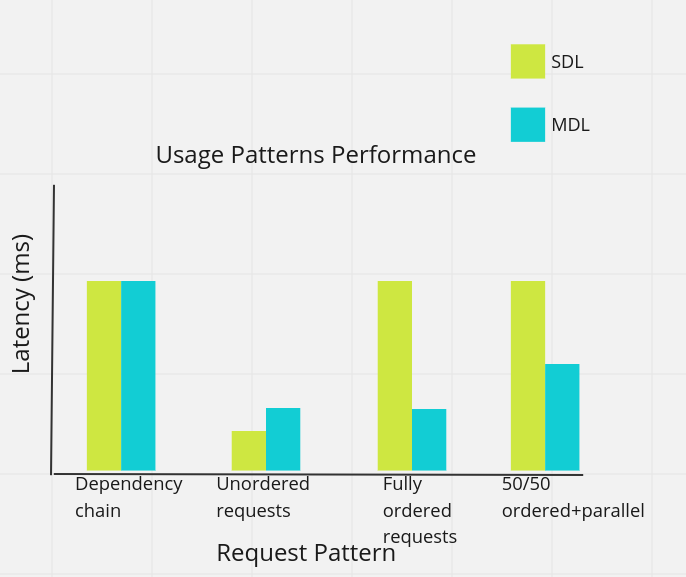
\includegraphics[scale=.32]{usage_patterns_perf.png}
\caption{We break down for which request types MDL can provide a speedup compared to SDL.}
\label{fig:usage}
\end{figure}
\subsubsection{Real Application}
Run some application on top of a SDL kv-store and then on top of a MDL kv-store, and compare the e2e application level throuhgput. It would be doubly interesting if different request types can be measured independently to see which ones have a wider speedup than others, and then look at how they work and answer why.

We probably won't get around to this for an MVP.

Some applications to consider:
\begin{itemize}
    \item Facebook web-server
    \item Banking app
    \item Music listening app
\end{itemize}
\subsection{Evaluation notes to self}
\begin{itemize}
    \item single shard: consider issues with whether to sort the per-client buffered requests or don't need to sort
    \item single/multi shard -- leader election? wb inconsistencies during leader failure, should voting take into account expectedSeqNo?
    \item Read leases
    \item how to simulate lossy network/reordering of messages being received at the system (per client)?
\end{itemize}